\subsection*{Mini-Paper}
\addcontentsline{toc}{subsection}{Mini-Paper}

\subsubsection*{Introduction}
\addcontentsline{toc}{subsubsection}{Introduction}

Multi-agent reinforcement learning (MARL) has garnered significant 
attention in recent years due to its potential to solve complex, 
collaborative, and competitive tasks across various domains. 
The extension to heterogeneous-agent reinforcement learning (HARL) 
further broadens the scope by incorporating diverse agents with 
differing capabilities and roles. As the field progresses, 
a critical area of research lies in understanding how different 
MARL and HARL algorithms perform under varying conditions, 
such as changes in the number of participating agents.

This paper presents an experimental study that evaluates several 
state-of-the-art MARL and HARL algorithms under dynamic conditions 
where the number of agents changes between training and deployment. 
The primary aim is to establish a comparative baseline for the 
performance and robustness of these algorithms, contributing to the 
body of knowledge on their practical applicability and effectiveness. 
By replicating and contrasting the results reported by the original 
authors of these algorithms, this study seeks to either corroborate or 
challenge existing findings, thereby enhancing the reliability of 
performance benchmarks in MARL and HARL.

Furthermore, this experiment investigates the resource costs 
associated with the initial training phases of these algorithms. 
Understanding the computational and time resources required to 
achieve optimal performance under standard conditions is crucial 
for deploying these algorithms in real-world applications. 
Additionally, we assess the resource implications of adapting the 
algorithms to maintain benchmark performance when the number of agents 
changes during deployment. This dual focus on initial training and 
adaptive performance evaluation provides a comprehensive view of the 
efficiency and scalability of current MARL and HARL approaches.

Through this examination, we aim to highlight the strengths and weaknesses 
of the tested algorithms, offering insights into their suitability for 
different multi-agent environments. The findings from this study are 
expected to inform future research and development in the field, 
guiding improvements in algorithm design and deployment strategies.

%\section{Related Work}
\subsubsection*{Related Work}
\addcontentsline{toc}{subsubsection}{Related Work}

The field of multi-agent reinforcement learning (MARL) and its extension 
to heterogeneous-agent reinforcement learning (HARL) has seen significant 
advancements over the past decade. 
This section reviews the key literature relevant to our study,

DeepMind's development of AlphaGo \cite{silver2016} and subsequent iterations, 
AlphaGo Zero \cite{silver2017} and AlphaStar \cite{vinyals2019}, demonstrated 
the power of deep reinforcement learning in multi-agent environments. 
These models, particularly AlphaStar, which operates in the complex, 
dynamic environment of StarCraft II, highlight the scalability and 
effectiveness of MARL algorithms. 
They provide an example of what is achievable, albeit with substantial 
resources of a scale unavailable to the vast majority of researchers or
other organizations.
In response, there have been numerous efforts to improve 
efficiency at various levels of training.

%%

Smit et al.~\cite{smit2023} focused on leveraging scalability
to reduce training requirements. They used a simulated football 
environment which, at full scale, uses two teams of 11 agents.
They explored extensions of the PPO algorithm to attempt to 
produce an effective team of 11 agents, while training only 4.
Ultimately they were unable to achieve the performance that they sought.
In their work they did not address why PPO was selected over any other
algorithm.

\textbf{Algorithms:}

Lowe et al.~\cite{lowe2020} observed weaknesses in Q-learning and policy
gradient methods when applied to multi-agent settings. They proposed
an algorithm that they called multi-agent deep-deterministic policy-gradient
(MADDPG), which extends a single agent DDPG~\cite{lillicrap2019}
with a shared critic.

Multi-agent Twin Delayed Deep Deterministic policy gradient (MATD3)~
\cite{ackermann2019} extends TD3~\cite{fujimoto2018}, also using a 
shared critic.

Multi-agent Trust Region Policy Optimization (MATRPO)~\cite{li2023c}
extends TRPO~\cite{schulman2017} using a shared likelihood
ratio on action optimality that has the advantage of preserving
privacy of each agent's own policy.

Multi-agent Proximal Policy Optimization (MAPPO)~\cite{yu2022} extends
PPO~\cite{schulman2017a} through shared parameters.

Importance Weighted Actor-Learner Architecture (IMPALA)~\cite{espeholt2018}
is an algorithm with a central learner but with highly decentralized 
execution, that supports homogeneous multi-agent applications from the
original implementation.

Zhong et al.~\cite{zhong2024} proposed a suite of algorithms,
which extend MADDPG, MATD3, MATRPO, and MAPPO,
to be more flexible with the agents that they are applied to.
They sought to improve the efficiency of training agents capable
of cooperation through changes to the original algorithms that 
emphasized development of distinct behavior.

They called their modified MARL algorithms, heterogeneous-agent 
reinforcement learning (HARL).
Though the agents themselves are not heterogeneous,
the algorithms are written to encourage the development of
heterogeneous policies and behavior.
Along with their paper, Zhong et al.~\cite{zhong2024} do provide the code 
that they used to implement their algorithms and perform their experiments.
Their experiments evaluated each of their algorithms against the algorithm 
that it was based when trained in six common baseline environments.


\textbf{Environments:}

Gupta et al.~\cite{gupta2017cooperative} published a set of cooperative 
tasks for evaluating MARL algorithms. Collectively they are sometimes
referred to as the SISL (Stanford Intelligent Systems Laboratory)
environments. The environments included in the SISL benchmarks
are called Multiwalker, Pursuit, and Waterworld.
Each provide a distinct task that requires cooperation and they
have parameters that allow the number of agents instantiated to be changed. 

\phantom{\hfil} % Fix under full box

\emph{Other environments to be described as they are implemented...}


%\section{Methodology}
\subsubsection*{Methodology}
\addcontentsline{toc}{subsubsection}{Methodology}

This section describes the experimental methodology used to
evaluate the selected algorithms. 

\phantom{\hfil} % Fix under full box

\textbf{Fixed Agent Count Training:}
Each algorithm was trained with several different fixed numbers of agents. 
The training process followed the protocols and hyperparameters 
recommended by the authors of the respective algorithms. 
Training was conducted over 200 episodes.

Performance metrics such as cumulative rewards, wall-clock training time,
CPU utilization, and memory utilization are collected during this training
period, and will relate directly to previously reported metrics claimed
in other works.

\textbf{Evaluation Under Altered Conditions:}
After initial training, the agents are evaluated on the task with
and altered team size. Specifically, we tested each model with both 
fewer and more agents than were present during training. 
The variations included incremental increases and decreases in the 
agent count to observe performance trends.

\textbf{Adaptive Training:}
During this step we resume the training of the team of agents
under the new environmental conditions.
In doing so we seek to evaluate both the feasibility of this
method of retraining, and to determine if there are resource benefits
when compared to training an entirely new set of agents with the 
expected team size.

\phantom{\hfil} % Fix under full box

\textbf{Waterworld:}
This environment implements a task that simulates small organisms
that must cooperate to gather food items and avoid poisoned items.
Each agent has a range limited, 212-dimension observation space.
By default they are rewarded \(+10\) for successful cooperation and 
consumption of a food item, and \(-1\) for colliding with a poisoned
item. For reward shaping a \(+0.1\) is given to each agent when they 
collide with a food item, independent of if they are able to consume it.

The principle variables that we use in this experiment are the number of
agents in the environment, and the number of agents that are need to 
cooperatively consume a food item.

\phantom{\hfil} % Fix under full box

\textbf{Multiwalker:}
This environment is an extension of the Farama gymnasium bipedal walker.
It consists of several bipedal walkers with a long box placed upon their head.
The action space for the walkers consists of changing the angles of their 
leg joints. Each walker has an observation space that is 32-dimensional 
and represents a noisy lidar reading of the area in front of the walker.
The range is limited enough that they are only able to observe up to two 
walkers in front of themselves. 
Dropping the package nets a reward of \(-100\), 
and moving the package forward rewards \(+1\).

Although it was not emphasized by the authors, the walkers themselves
are homogeneous in capability, but their positioning does create 
heterogeneous observation spaces, and potentially functionality;
particularly for the first two walkers compared to the rest.

This is taken into account during the evaluation with differing team size,
when the agents have distinct policies.
Because three is the minimum number of walkers that the environment
supports, the first two always remain the first two. 
The change in team size is achieved by randomly adding copies selected from 
the third or greater agent, to increase the team size; or randomly omitting
an agent third or greater to reduce the team size.

%\section{Results}
\subsubsection*{Early Results}
\addcontentsline{toc}{subsubsection}{Early Results}

\textbf{Waterworld:}

Preliminary results (\cref{fig:ww_base_2co}) show that unsurprisingly,
PPO does reliably converge on increasingly effective policies.
Additionally, it also appears that there is an inflection point 
at which increasing the number of agents reduces the total return.
This is too small of a sample to draw meaningful conclusions but it 
does suggest that we will want to be aware that such an inflection point
may exist. For the environment where the cooperation parameter is set to 2,
it appears that somewhere around 4 or 5 agents achieves maximum performance. 
Below this point it is likely that the agents are too few to effectively 
accomplish the task, 
and above this point the agents begin to compete and that there are too
few objectives, while increasing the collisions that result in negative
returns.

\begin{figure}
    \centering
    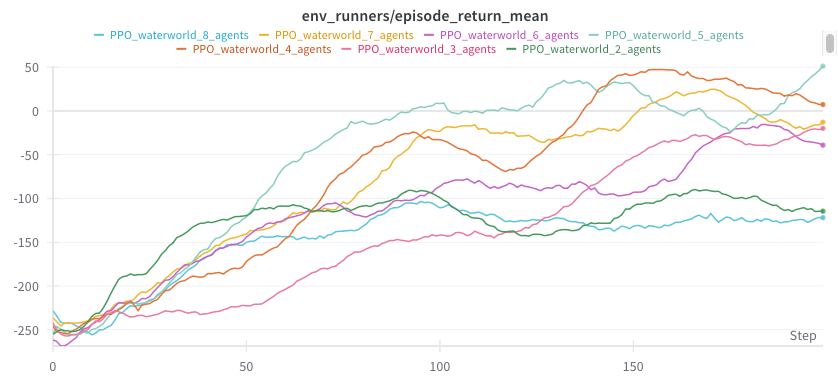
\includegraphics[width=.9\linewidth]{waterworld_base_coop_2.png}
    \caption{Mean Training Episode Return for Waterworld (Coop=2)}
    \label{fig:ww_base_2co}
\end{figure}

\textbf{Multiwalker:}

The first runs of Multiwalker returns (\cref{fig:walker_base})
show earlier and faster improvements with fewer agents,
but over a longer training period, the greater number of agents
net a higher reward.
It should be noted that the positive return for this task is the same for 
each agent, but it is added to each agent's individual score.
The negative for dropping the box is also given to all agents.
The penalties for an agent falling or moving its head to an extreme 
angle are added only to that agent's score.

\begin{figure}
    \centering
    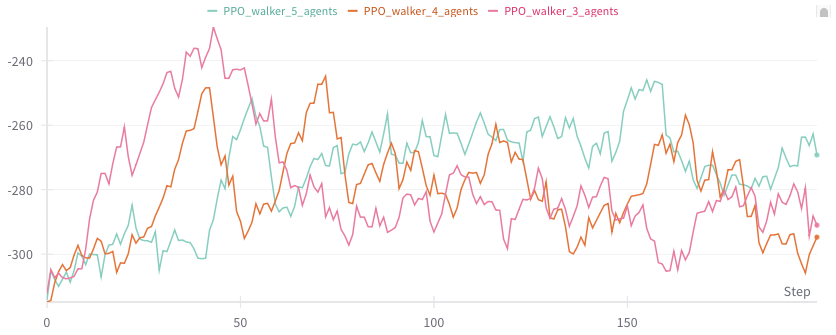
\includegraphics[width=.9\linewidth]{walker_base.png}
    \caption{Mean Training Episode Return for Multiwalker}
    \label{fig:walker_base}
\end{figure}


\subsubsection*{Future Work}
\addcontentsline{toc}{subsubsection}{Future Work}
\emph{
    After this exam has been turned in, work will continue on the subject of
    this mini-paper. The intended contribution will include a framework
    to allow others to replicate the results of this paper, 
    and be built in a manner that should be easier for others to use
    the constituent parts and tools that are currently being developed.
    Additionally, none of the HARL algorithms have been implemented in 
    either of the most common frameworks, and thus implementations
    built for this experiment will be the subject of a pull request
    to the contribution branch of RLlib.
}

%\section{Conclusion}
%\section{Bibliography}